\documentclass[12pt]{article}
 
\usepackage[margin=1in]{geometry} 
\usepackage{amsmath,amsthm,amssymb}
\usepackage{graphicx}
 
\newcommand{\N}{\mathbb{N}}
\newcommand{\Z}{\mathbb{Z}}
\newcommand{\R}{\mathbb{R}}
\newcommand{\C}{\mathbb{C}}
 
 
\begin{document}
 
% --------------------------------------------------------------
%                         Start here
% --------------------------------------------------------------
 
\title{Solutions to Sheet 1}
\author{Leif Van Holland, 2nd author \\ \\
\textsc{Pattern Matching and Machine Learning} \\
\textsc{for Audio Signal Processing}}

\maketitle

\section*{Exercise 1.1}
\begin{itemize}
    \item[(a)] \[z = \left(1+i\sqrt{3}\right)^2 = 1+2i\sqrt{3}-3=-2+i(2\sqrt{3})\]
    
     \[\implies |z| = \sqrt{(-2)^2 + (2\sqrt{3})^2} = \sqrt{16} = 4\]
     
     With $\text{Re}[z] < 0$ and $\text{Im}[z] > 0$, we know that the point is in the upper left quadrant of the coordinate system. Therefore, $\varphi < \pi$.
     
     \[\cos \varphi = \frac{\text{Re}[z]}{|z|} = \frac{-2}{4} = -\frac{1}{2} \implies \varphi = \frac{2}{3}\pi\]
     
     \[\implies z = |z|\cdot \exp(i\varphi) = 4\cdot\exp(\frac{2\pi i}{3}).\]
     
     \item[(b)] \[z=\frac{e^{\frac{\pi}{3}i}}{e^{\frac{2}{3}\pi i}\cdot 2e^{\frac{\pi}{6}i}} = \frac{1}{2}e^{(\frac{1}{3}-\frac{2}{3}-\frac{1}{6})\pi i} = \frac{1}{2}e^{(\frac{-\pi}{2}i)} = 0-\frac{1}{2}i\]
     
     \item[(c)] \[\text{Re}\left[5e^{\frac{\pi}{2}i}+\sqrt{2}e^{\frac{\pi}{4}i} \right] = \text{Re}\left[5i + \sqrt{2}(\frac{1}{\sqrt{2}}+\frac{1}{\sqrt{2}}i)\right] = \text{Re}\left[ 1 + 6i \right] = 1\]
     
     \item [(d)] From Euler's Formula we know that for all $z\in\mathbb{C}$
     \[ \sin(z) = \frac{e^{iz}-e^{-iz}}{2i},\quad \cos(z) = \frac{e^{iz}+e^{-iz}}{2} \]
     We can conclude, that
     \begin{align*}
         \sin(z)^2 + \cos(z)^2 &= \left(\frac{e^{iz}-e^{-iz}}{2i}\right)^2 + \left(\frac{e^{iz}+e^{-iz}}{2}\right)^2 \\
         &= \frac{e^{2iz}-2e^{iz}e^{-iz}+e^{-2iz}}{-4} + \frac{e^{2iz}+2e^{iz}e^{-iz}+e^{-2iz}}{4} \\
         &= \frac{-e^{2iz}-e^{-2iz}+2}{4} + \frac{e^{2iz}+e^{-2iz}+2}{4} \\
         &= \frac{4}{4} = 1.
     \end{align*}
     
\end{itemize}

\section*{Exercise 1.2}
\begin{figure}[h]
    \centering
    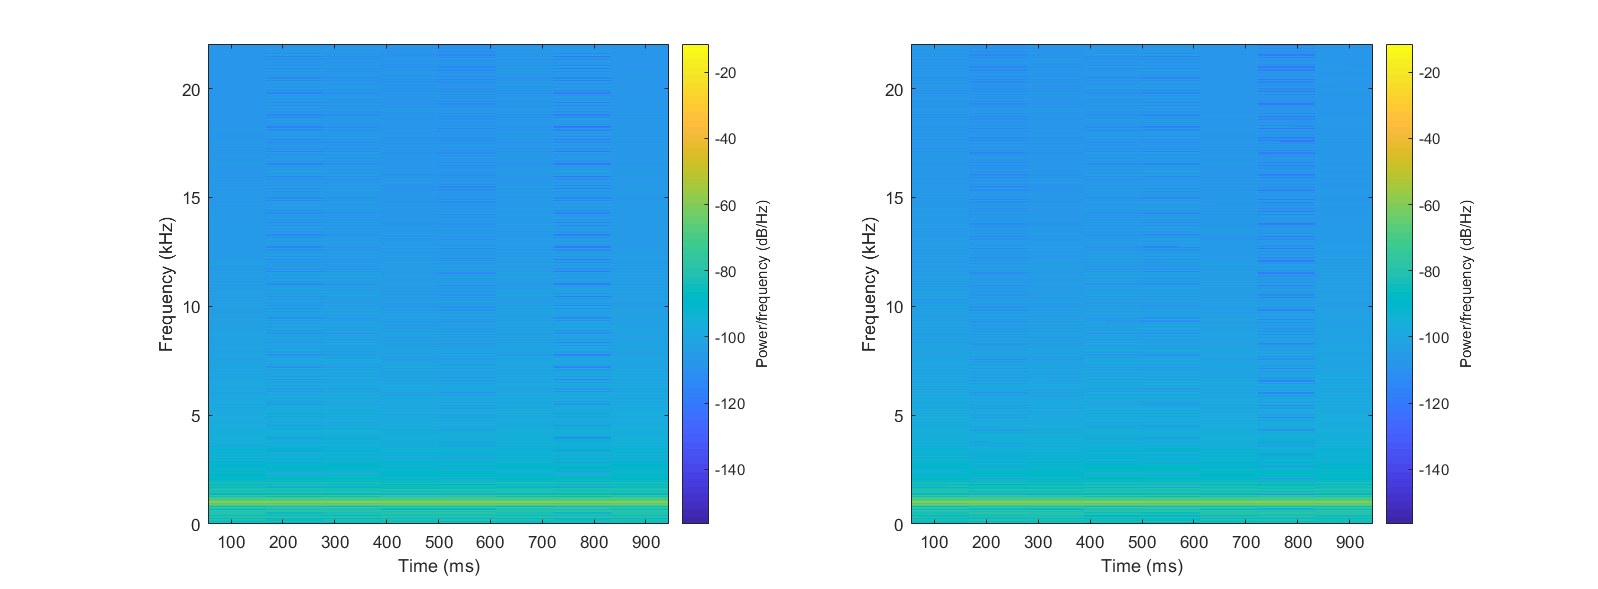
\includegraphics[width=\textwidth]{spectrograms}
    \caption{Spectrograms of a sine (left) and cosine (right) wave of frequency $f = 1000$ Hz.}
\end{figure}

\begin{itemize}
    \item [(c)] One can observe that there is no difference in the spectrograms of the two waves. This is due to the fact that the cosine wave is just a phase-shifted version of the sine wave:
    \[\cos(\varphi) = \sin\left(\varphi+\frac{\pi}{2}\right)\]
\end{itemize}
 
% --------------------------------------------------------------
%     You don't have to mess with anything below this line.
% --------------------------------------------------------------
 
\end{document}